\clearpage
\section{Sequence Diagram Design}

\subsection{Scenario Description}

The sequence diagram illustrates the interaction between the Smart Meter, Backend Server, Blockchain Smart Contract, Database, and Consumer during the prepaid billing process.

\subsection{Sequence Diagram}

Figure~\ref{fig:sequence} illustrates the chronological sequence of messages exchanged among system components.

\begin{figure}[H]
    \centering
    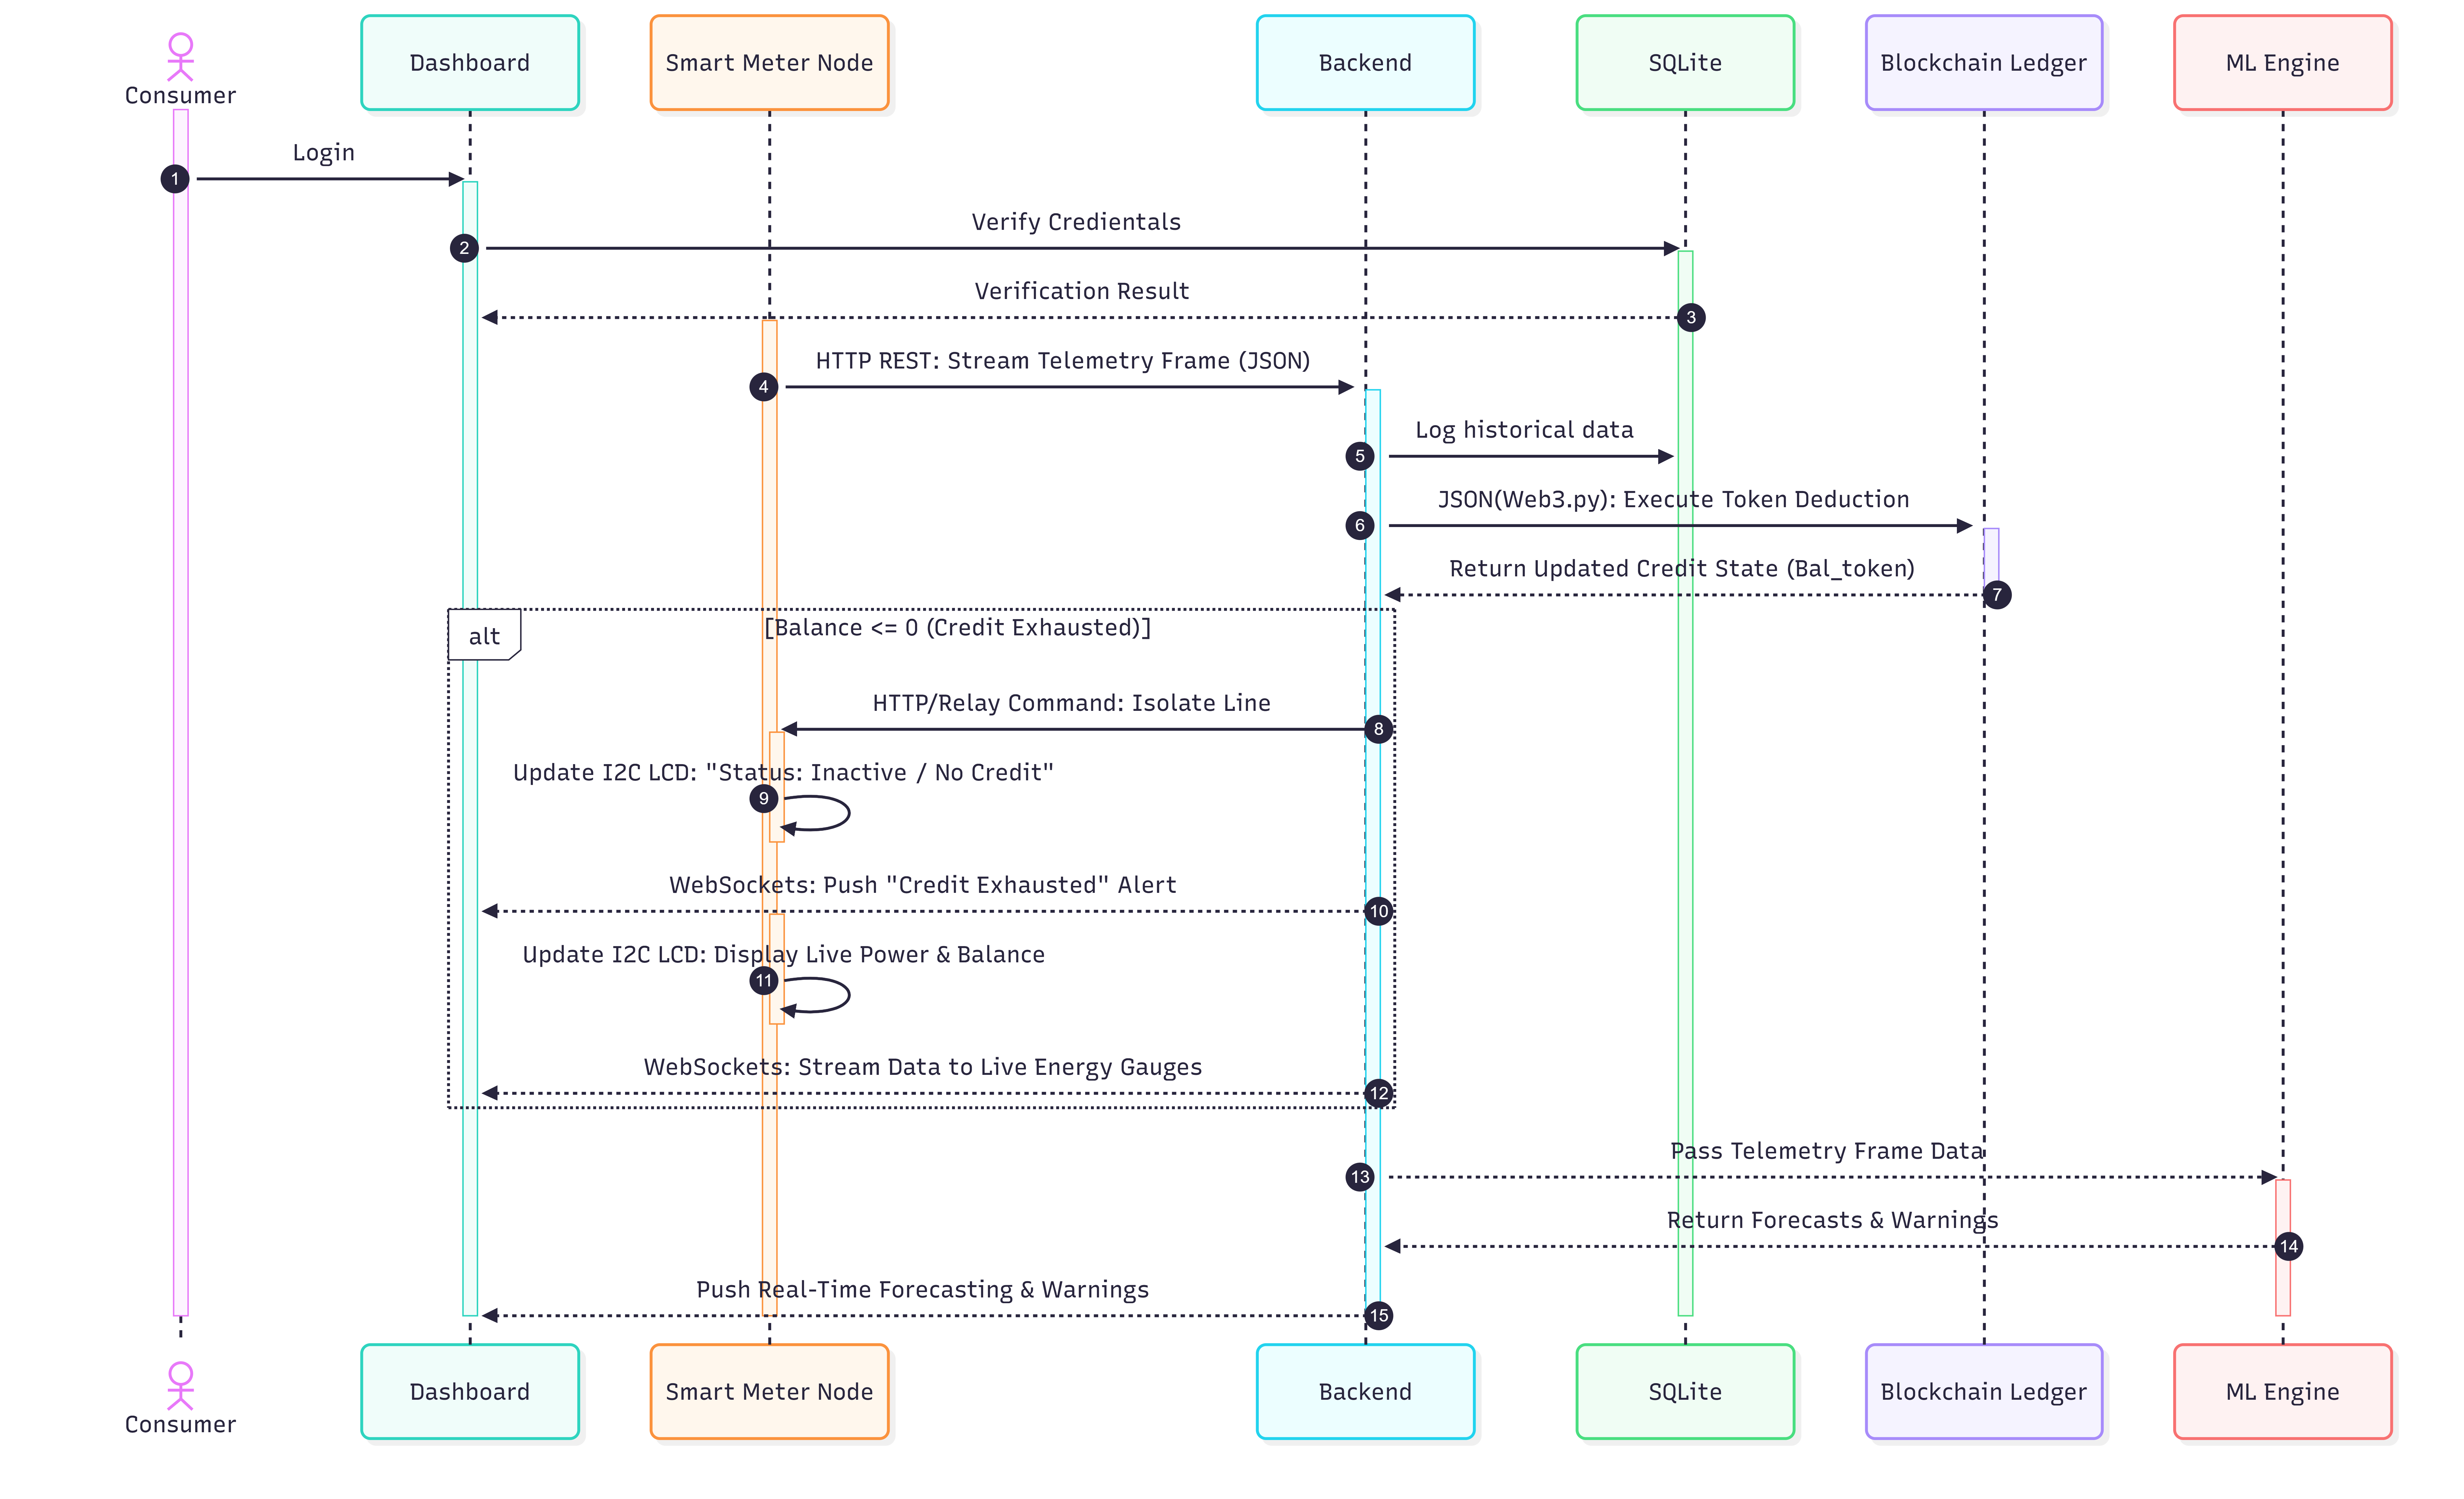
\includegraphics[width=\textwidth]{graphics/sequence diagram.png}
    \caption{Sequence Diagram of the Decentralized Smart Power Grid System}
    \label{fig:sequence}
\end{figure}

\subsection{Interaction Description}

The smart meter periodically transmits electricity consumption data to the backend. After validating the telemetry, the backend invokes the blockchain smart contract to deduct prepaid credit. The updated balance is stored in the database, and the dashboard is refreshed to provide real-time information to consumers and administrators.